% f2015hbw_q16_circle.tex — 2015 年高考数学·湖北卷·文科 第 16 题（圆与坐标轴）
%
% 【来源】`.work/phase3-b20/source/2015湖北文.pdf`（SHA-256
%   801e73338b6c4c747cc76b14e167d590a34e0b5a13a47719e5ee6cd4337e4cd2），
%   第 1 页（合订本页 953）；内容对象 5/7/9/…/19。逐路径实测见
%   `.work/phase3-b20/figure-inventory.md`。
%
% 【坐标口径】源 PDF 用户空间（原点左下、y 向上）。本图本地坐标
%   (x, y) = (x_page − 908.958, y_page − 653.476)，1 单位 = 1 TeX pt。
%   路径坐标逐点照录内容流（含三次贝塞尔控制点）。
%
% 元素计数：5 条路径（x/y 轴＋箭头、圆）＋8 个标签（含圆心点）
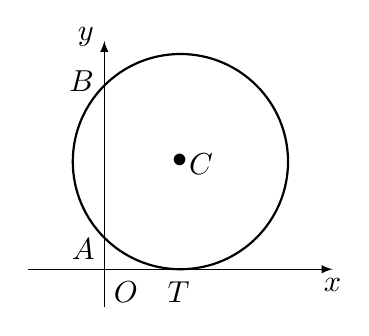
\begin{tikzpicture}[x=1pt, y=1pt,
    every node/.style={inner sep=0pt, font=\fontsize{10.5pt}{12.6pt}\selectfont}]
  \draw[line width=0.398pt] (-0.0004,13.7480)   -- (106.3986,13.7480);
  \fill[line width=1.0pt] (109.9853,13.7480)   .. controls (108.9223,13.9470) and (107.1953,14.5450) .. (106.0003,15.2420)   -- (106.0003,12.2540)   .. controls (107.1953,12.9510) and (108.9223,13.5490) .. (109.9853,13.7480);
  \draw[line width=0.398pt] (27.4960,-0.0002)   -- (27.4960,92.6508);
  \fill[line width=1.0pt] (27.4960,96.2373)   .. controls (27.2970,95.1743) and (26.6990,93.4473) .. (26.0020,92.2523)   -- (28.9900,92.2523)   .. controls (28.2930,93.4473) and (27.6950,95.1743) .. (27.4960,96.2373);
  \draw[line width=0.797pt] (93.8783,52.6339)   .. controls (93.8783,74.1099) and (76.4683,91.5199) .. (54.9923,91.5199)   .. controls (33.5163,91.5199) and (16.1063,74.1099) .. (16.1063,52.6339)   .. controls (16.1063,31.1579) and (33.5163,13.7479) .. (54.9923,13.7479)   .. controls (76.4683,13.7479) and (93.8783,31.1579) .. (93.8783,52.6339)   -- cycle;

  \node[anchor=center] at (20.842,97.614) {$y$};  % 源中心 (929.80,751.09)
  \node[anchor=center] at (19.292,81.564) {$B$};  % 源中心 (928.25,735.04)
  \node[anchor=center] at (19.892,21.064) {$A$};  % 源中心 (928.85,674.54)
  \node[anchor=center] at (35.242,5.464) {$O$};  % 源中心 (944.20,658.94)
  \node[anchor=center] at (54.292,5.464) {$T$};  % 源中心 (963.25,658.94)
  \node[anchor=center] at (109.942,8.164) {$x$};  % 源中心 (1018.90,661.64)
  \node[anchor=center] at (62.442,51.664) {$C$};  % 源中心 (971.40,705.14)
  \node[anchor=center] at (54.992,53.114) {$\bullet$};  % 源中心 (963.95,706.59)

\end{tikzpicture}
%
% 【自验结果】
%   探针：latexmk -pdfxe（待跑）。
